\documentclass[a4,10pt,zihao=-4]{ctexart}
\linespread{1.0} % 设置单倍行距

\usepackage{ctex}
\usepackage[utf8]{inputenc}
\usepackage{amsfonts,amsmath,amscd,amssymb,amsthm}
\usepackage{latexsym,bm}
\usepackage{cite}
\usepackage{mathtools,mathdots,graphicx,array}
\usepackage{fancyhdr}
\usepackage{lastpage}
\usepackage{color}
\usepackage{enumitem}
\usepackage{mpdoc}
\usepackage{diagbox}
\usepackage{xcolor,tcolorbox,tikz,tkz-tab,mdframed,tikz-cd}
\usepackage{framed}
\usepackage{verbatim}
\usepackage{extarrows}
\usepackage{fontspec}
\graphicspath{{./assets/}}  % 设置图片的默认路径

\begin{document}
\pagenumbering{roman}
\title{实验四\,\,\,\,综合应用设计—交通灯控制器}

\author{李雨轩 2204112913 计算机2205}
\date{2024年6月}
\maketitle

\section{实验目的}
\begin{enumerate}
  \item 掌握Verilog语言框架,编程及调试的方法。
  \item 熟悉Verilog的基本语法。
  \item 掌握Vivado开发平台及FPGA开发板的使用。
\end{enumerate}

\section{实验内容}
\begin{enumerate}
    \item 设计制作一个数字钟/交通灯控制器;
    \item 对电路进行RTL电路分析、代码分析和仿真分析 (仿真时不接入时钟分频模块) ;
    \item 下载到FPGA板卡做硬件验证测试;
    \item 验收通过后,撰写实验报告。
\end{enumerate}

\section{实验要求}
\begin{enumerate}
  \item 设计一个由一条主路和一条支路汇合成的十字路口交通灯控制器 (EGo1开发板) 
  \item 基础功能:
  \begin{enumerate}
      \item 主、支路各设三个LED灯,分别代表红、黄、绿灯;
      \item 主、支路各设置两个显示数码管,倒计时显示;
      \item 信号灯变换次序:主路绿灯、支路红灯30秒->主路黄灯、支路红灯5秒->主路红灯、支路绿灯20秒->主路红灯、支路黄灯5秒。
  \end{enumerate}
  \item 高级功能:
  \begin{enumerate}
      \item 夜间模式 (开关控制指示灯黄灯闪烁)  ;
      \item 手动调整信号灯时长。
  \end{enumerate}
\end{enumerate}

\section{实验过程及结果分析}

\subsection{交通灯控制器模块设计框图}
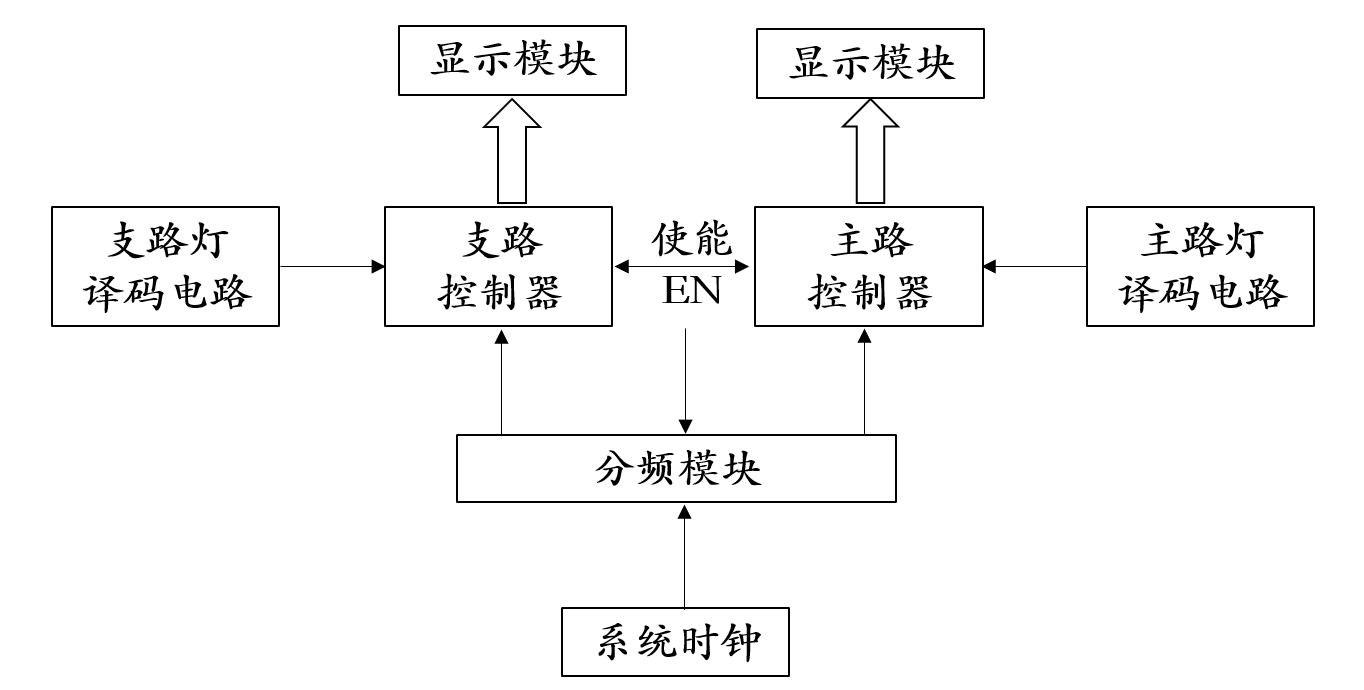
\includegraphics[width=0.8\textwidth]{module_analze.png}

\subsection{编写交通灯控制器Design Code}
\subsubsection{顶层模块 (traffic\_top)}
traffic\_top 模块是交通灯控制系统的顶层模块,它整合了多个子模块来实现交通灯的完整控制功能。其主要功能包括:时钟分频,即将输入时钟 clk 分频为 1Hz 时钟 clk\_1s;交通灯控制,即控制主路和支路的交通灯状态(红、黄、绿灯);倒计时显示,即显示主路和支路的倒计时;LED 驱动,即驱动主路和支路的交通灯 LED 显示;数码管显示,即控制数码管显示倒计时数字。

\vspace{1em}
\noindent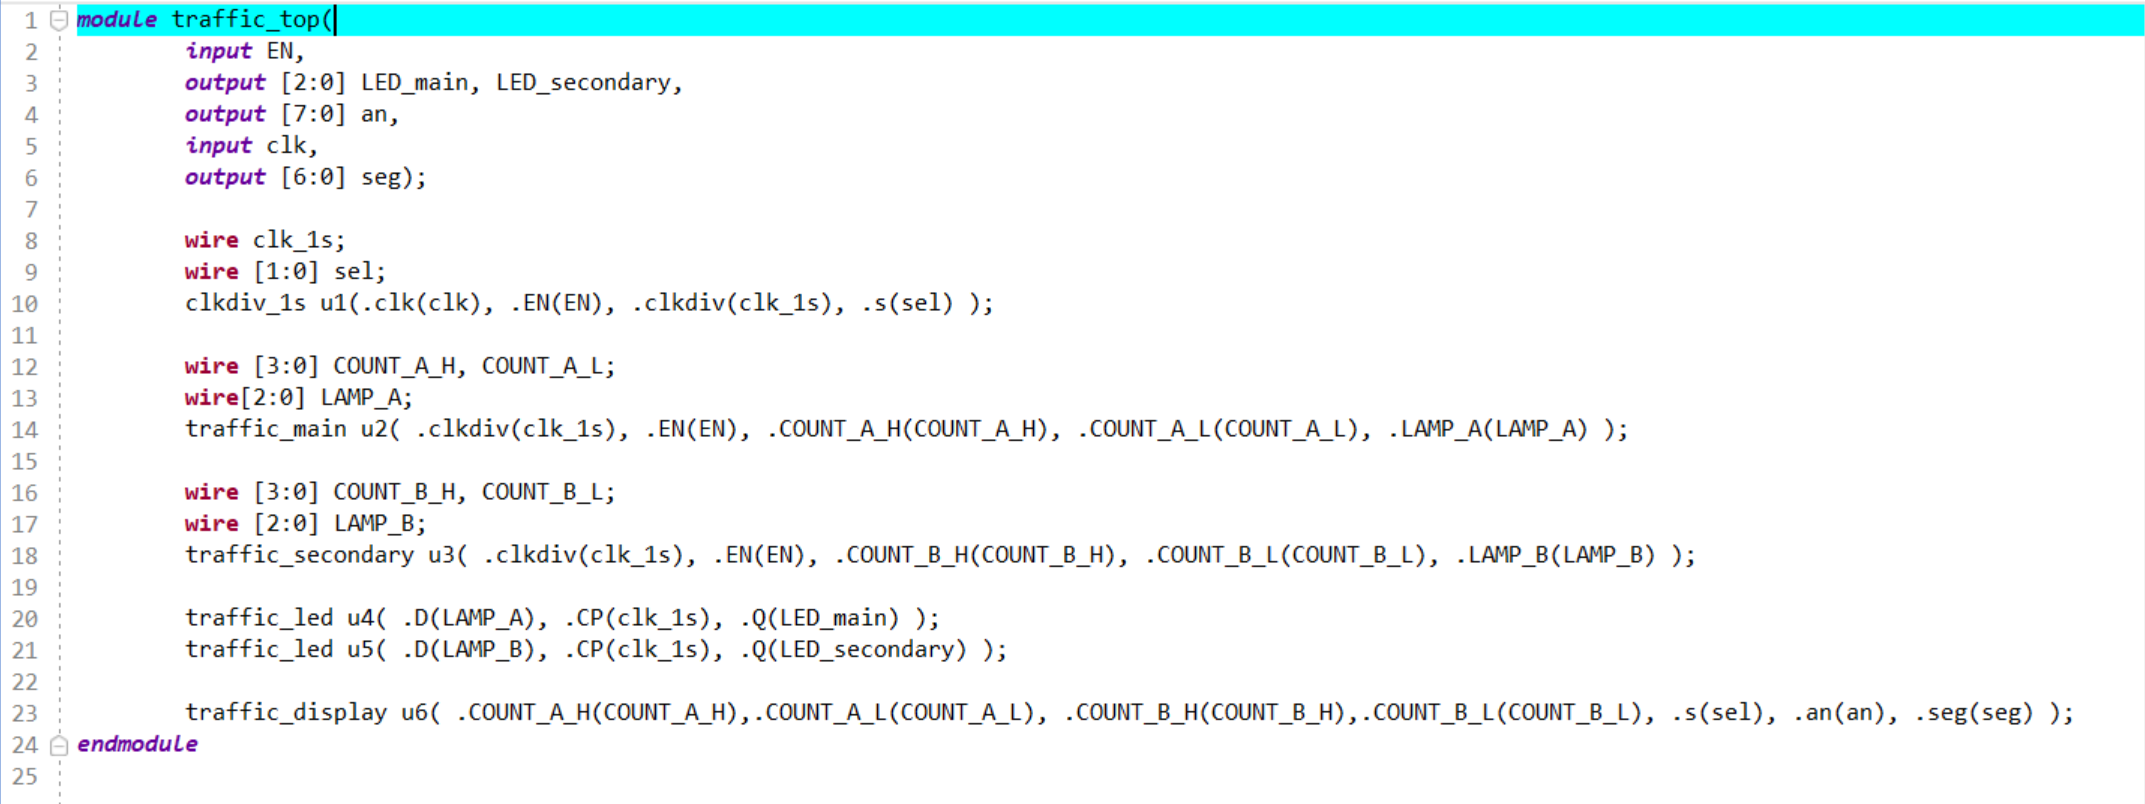
\includegraphics[width=1\textwidth]{traffic_top_code.png}


\newpage
\subsubsection{主路交通灯控制模块 (traffic\_main)}
traffic\_main 模块控制主路的交通灯状态,并在每个状态下执行倒计时功能。它通过时钟信号 clkdiv 和使能信号 EN 来控制交通灯的变换,并将倒计时的高位和低位数值分别输出到 COUNT\_A\_H 和 COUNT\_A\_L,交通灯的状态通过 LAMP\_A 输出。

\vspace{1em}
\noindent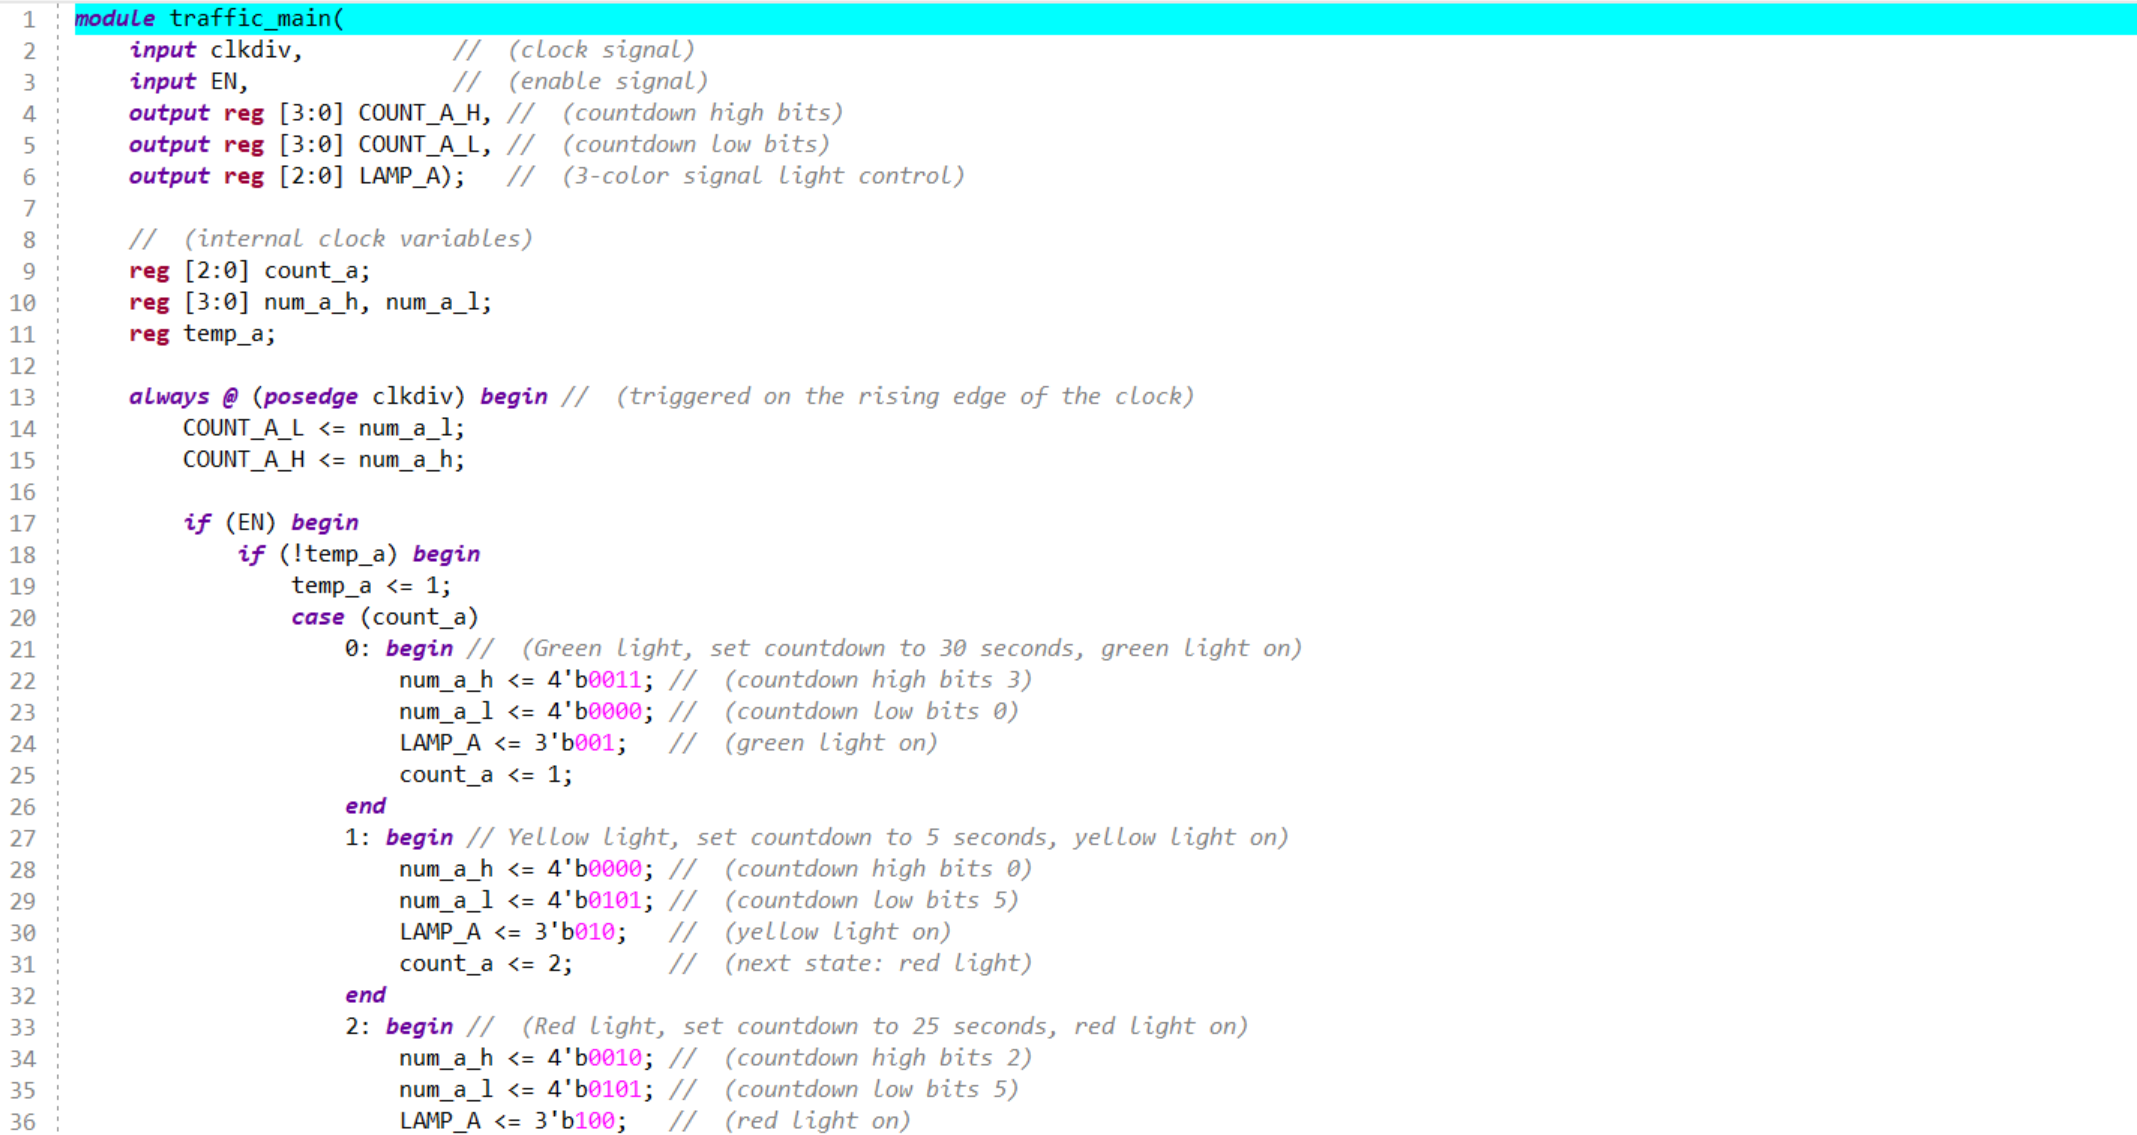
\includegraphics[width=1\textwidth]{traffic_main_1_code.png}
\noindent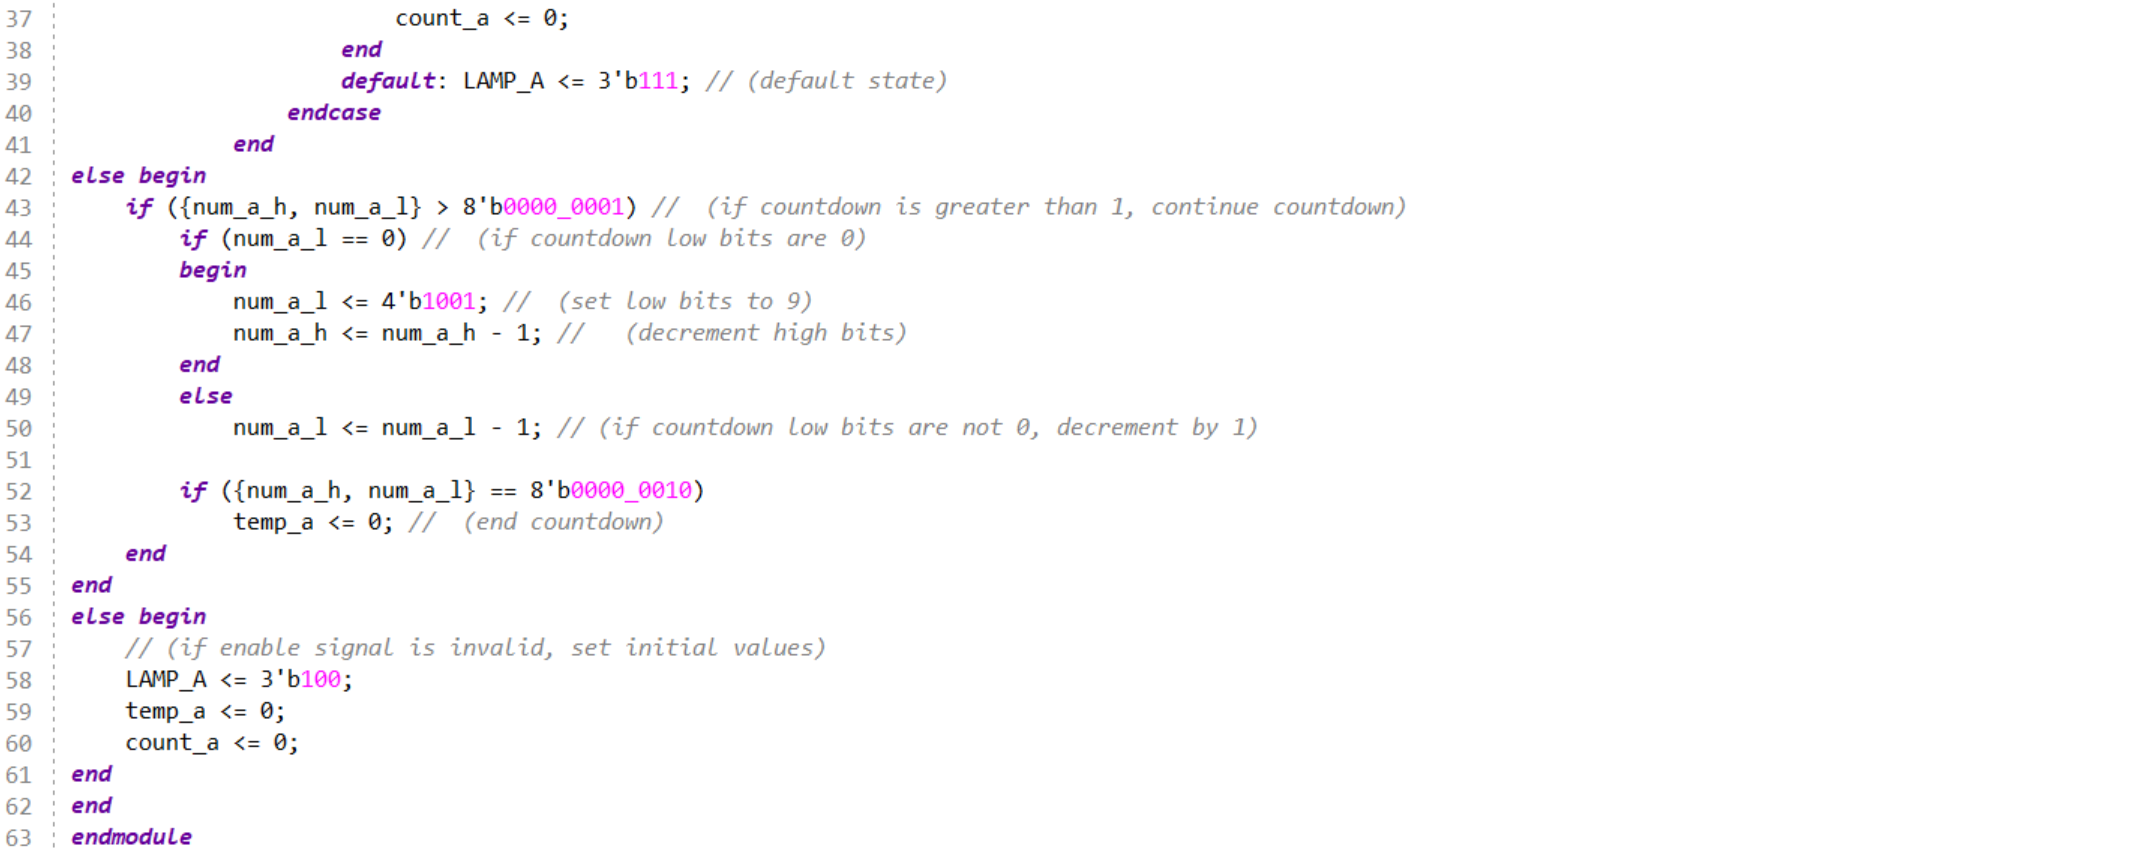
\includegraphics[width=1\textwidth]{traffic_main_2_code.png}


\newpage
\subsubsection{支路交通灯控制模块 (traffic\_secondary)}
traffic\_secondary 模块用于控制支路的交通灯状态,并在每个状态下执行倒计时功能。它通过时钟信号 clkdiv 和使能信号 EN 来控制交通灯的变换,并将倒计时的高位和低位数值分别输出到 COUNT\_B\_H 和 COUNT\_B\_L,交通灯的状态通过 LAMP\_B 输出。

\vspace{1em}
\noindent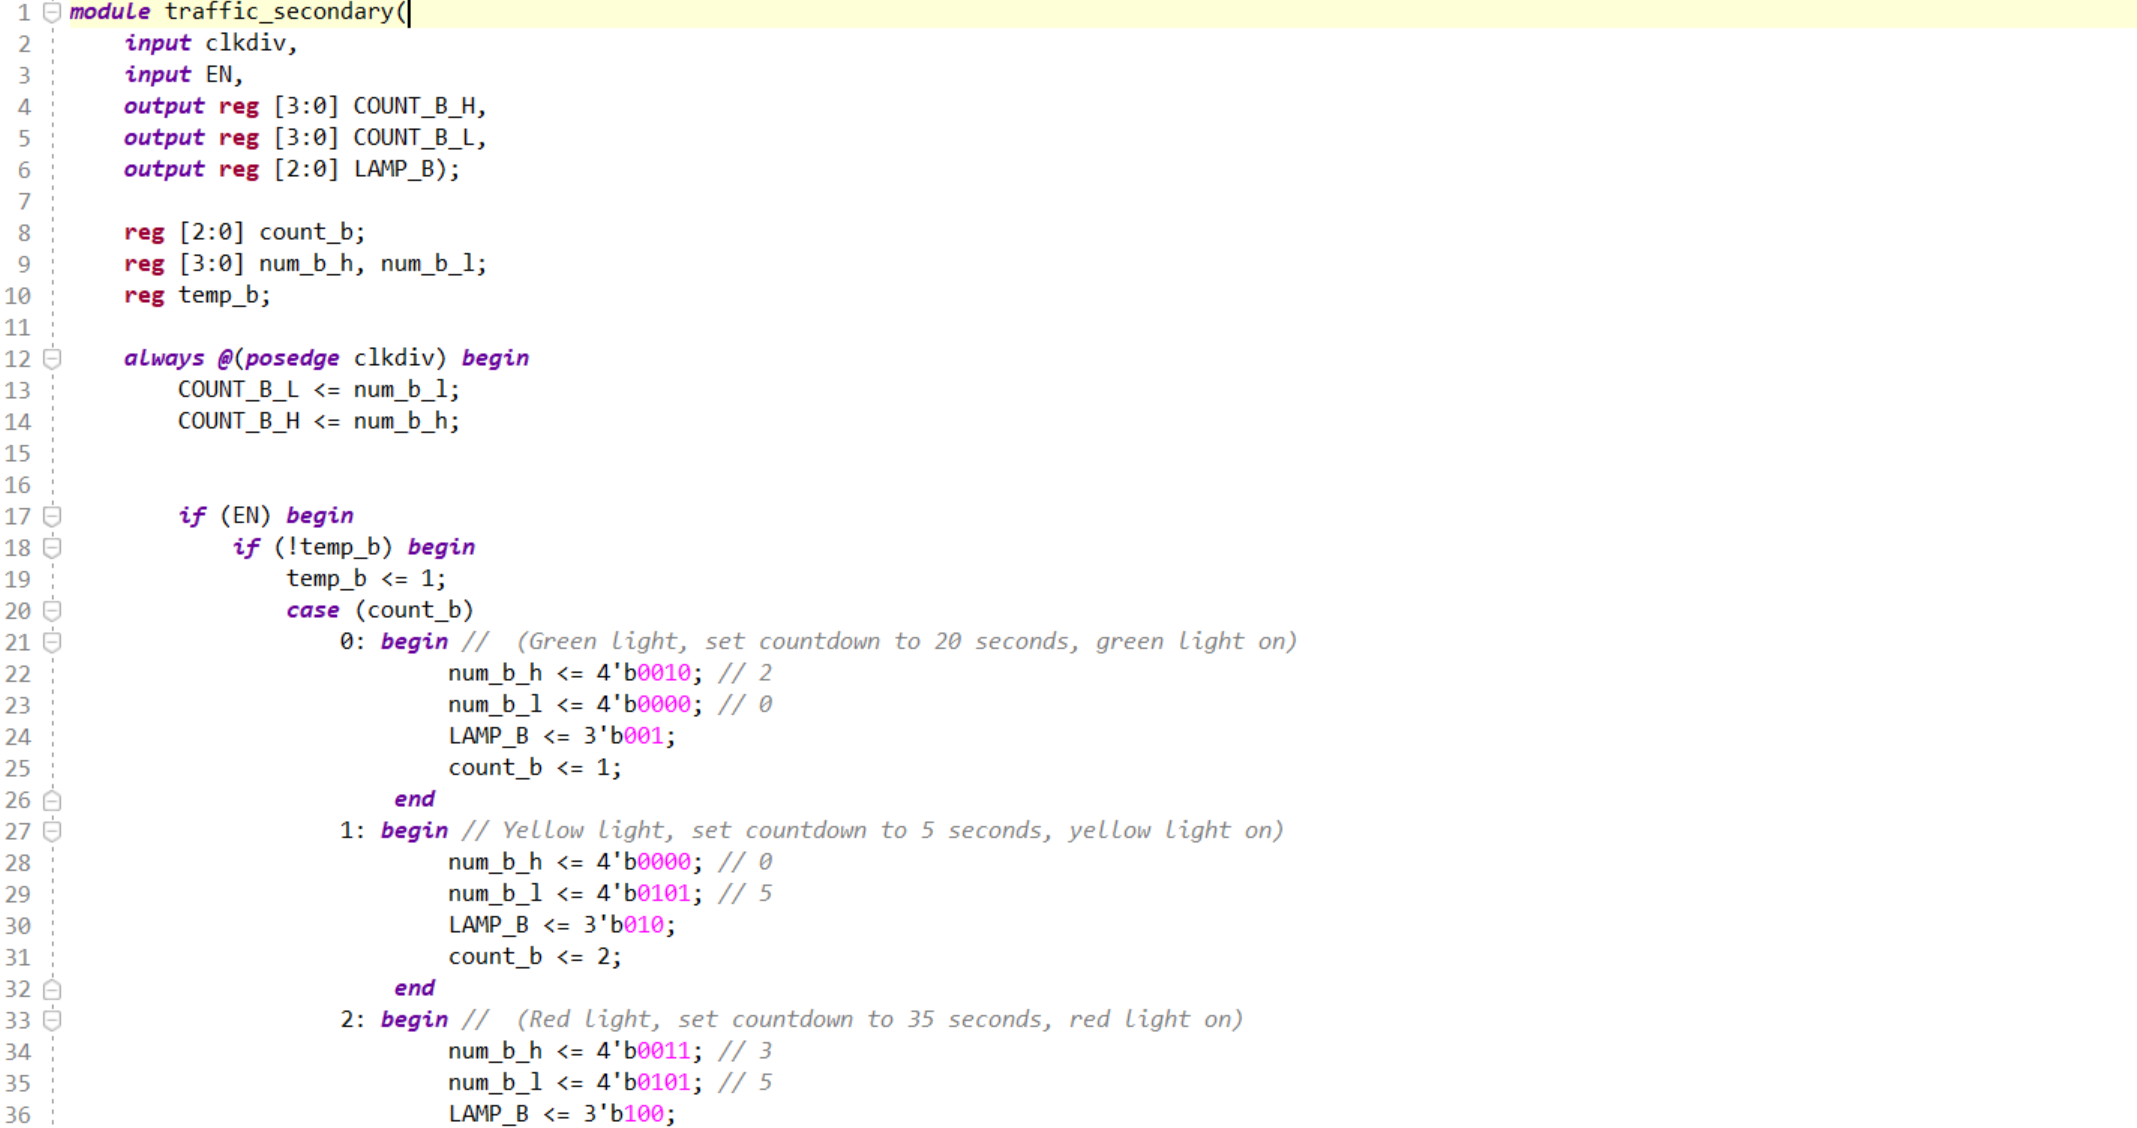
\includegraphics[width=1\textwidth]{traffic_secondary_1_code.png}
\noindent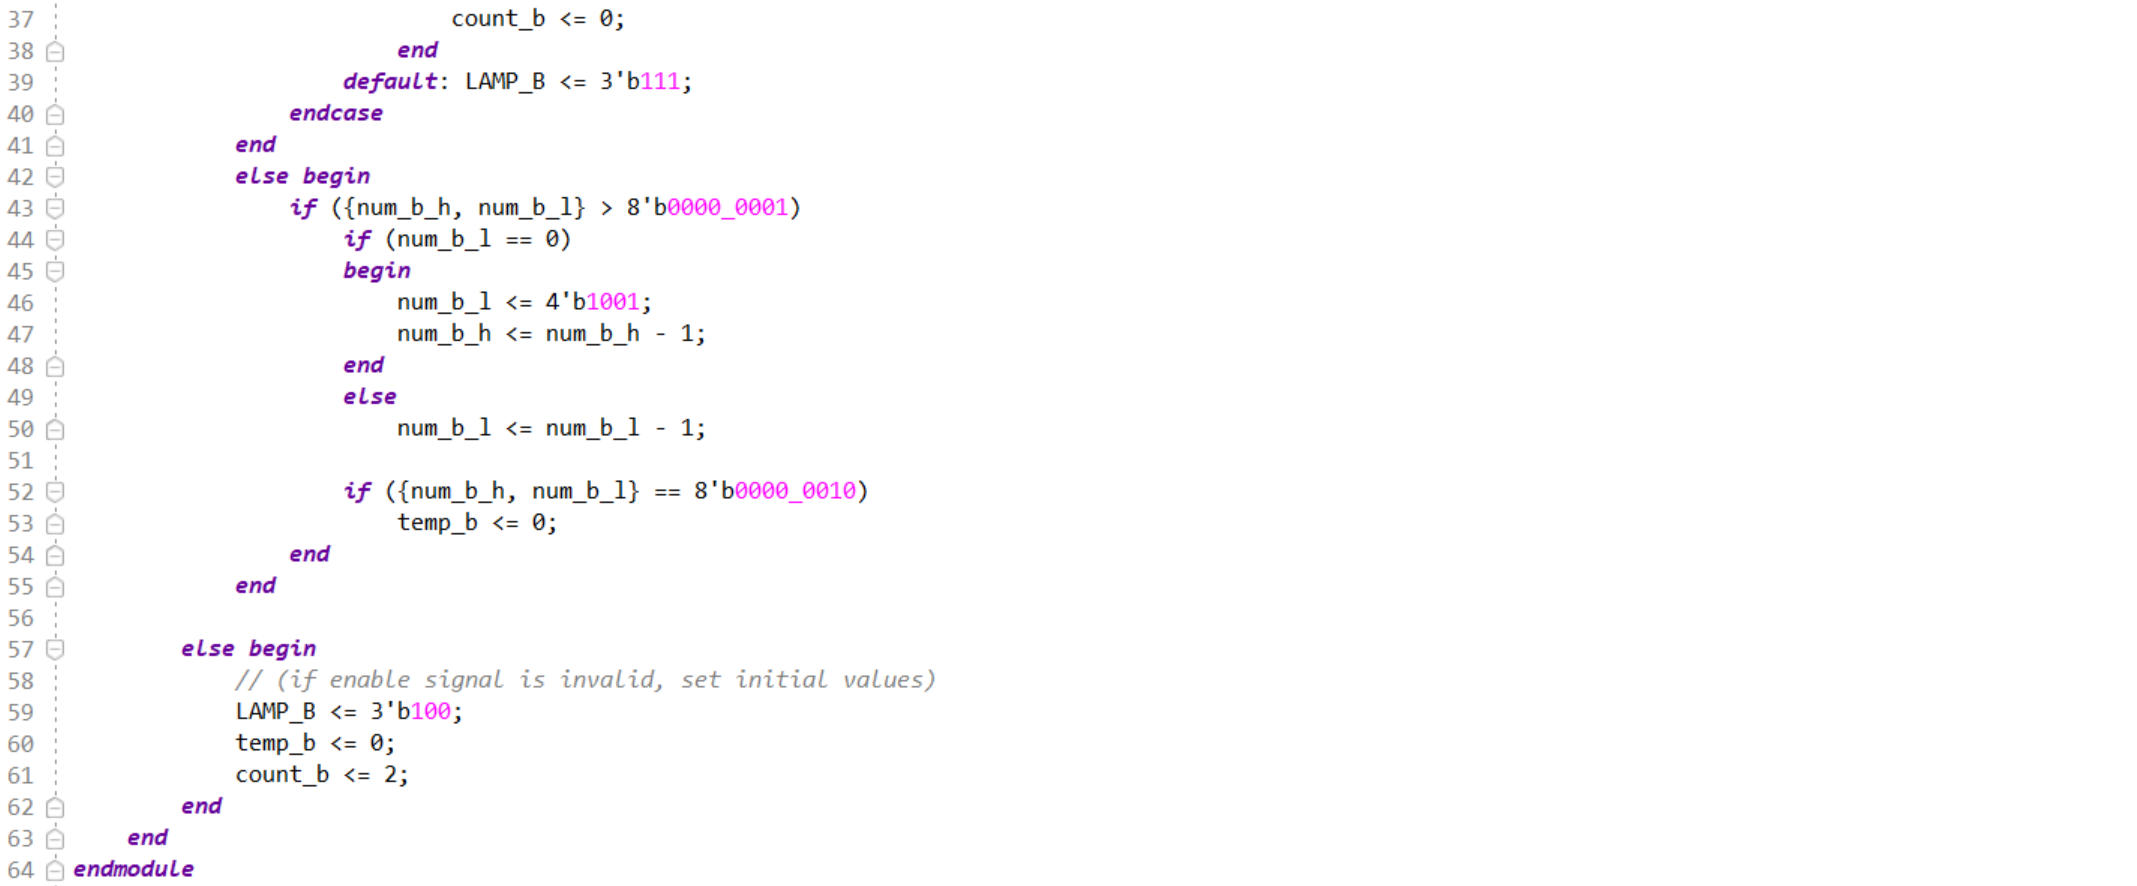
\includegraphics[width=1\textwidth]{traffic_secondary_2_code.png}

\subsubsection{对交通灯控制模块的分析}
上面这两个模块实现了主路和支路交通灯的控制和倒计时功能,每次倒计时结束后,交通灯状态按照绿灯、黄灯、红灯的顺序循环。 (下面的COUNT\_A\_H、num\_a\_h等也可替换为COUNT\_B\_H、num\_b\_h)

\begin{enumerate}
  \item 输入和输出及内部变量:
  \begin{enumerate}
      \item  clkdiv : 输入时钟信号,用于控制状态变化的时间间隔。
      \item  EN : 使能信号,控制模块的启用和禁用。
      \item  COUNT\_A\_H ,  COUNT\_A\_L : 输出倒计时的高位和低位数值。
      \item  LAMP\_A : 输出主路的交通灯状态。
      \item  count\_a : 用于跟踪当前的交通灯状态(绿灯、黄灯、红灯)。
      \item  num\_a\_h ,  num\_a\_l : 用于存储倒计时的高位和低位数值。
      \item  temp\_a : 用于控制倒计时的开始和结束。
  \end{enumerate}
  \item 工作原理:
  \begin{enumerate}
      \item 在时钟信号  clkdiv  的上升沿触发  always  块。
      \item 根据  EN  使能信号控制模块是否工作。
      \item 如果倒计时未开始( temp\_a  为 0),根据当前状态( count\_a )设置倒计时的初始值和交通灯状态。
        \begin{enumerate}
            \item 绿灯状态( count\_a == 0 ):倒计时设置为 30 秒,高位为 3,低位为 0,绿灯亮。
            \item 黄灯状态( count\_a == 1 ):倒计时设置为 5 秒,高位为 0,低位为 5,黄灯亮。
            \item 红灯状态( count\_a == 2 ):倒计时设置为 25 秒,高位为 2,低位为 5,红灯亮。
        \end{enumerate}
      \item 如果倒计时已开始( temp\_a  为 1),倒计时递减。
        \begin{enumerate}
            \item 如果低位为 0,高位减 1,低位设置为 9。
            \item 如果低位不为 0,低位减 1。
            \item 如果倒计时结束( {num\_a\_h, num\_a\_l} == 8'b0000\_0010 ),重置  temp\_a  为 0,倒计时结束。
         \end{enumerate}
  \end{enumerate}

\end{enumerate}


\subsubsection{LED 驱动器模块 (traffic\_led)}
traffic\_led 模块主要功能是状态传递,即在时钟信号 CP 的上升沿触发状态更新,将交通灯的状态信号 D 传递给输出信号 Q,用于驱动LED灯。

\vspace{1em}
\noindent\includegraphics[width=1\textwidth]{traffic_LED\_code.png}



\subsubsection{时钟分频器模块 (clkdiv\_1s)}
clkdiv\_1s 模块有两个功能,第一个是时钟分频,即将输入的高频时钟信号 clk 分频为1秒的时钟信号 clkdiv,供其他模块使用。另一个是状态信号,即生成2位的状态信号 s,供其他模块实现交通灯的状态控制逻辑。

\vspace{1em}
\noindent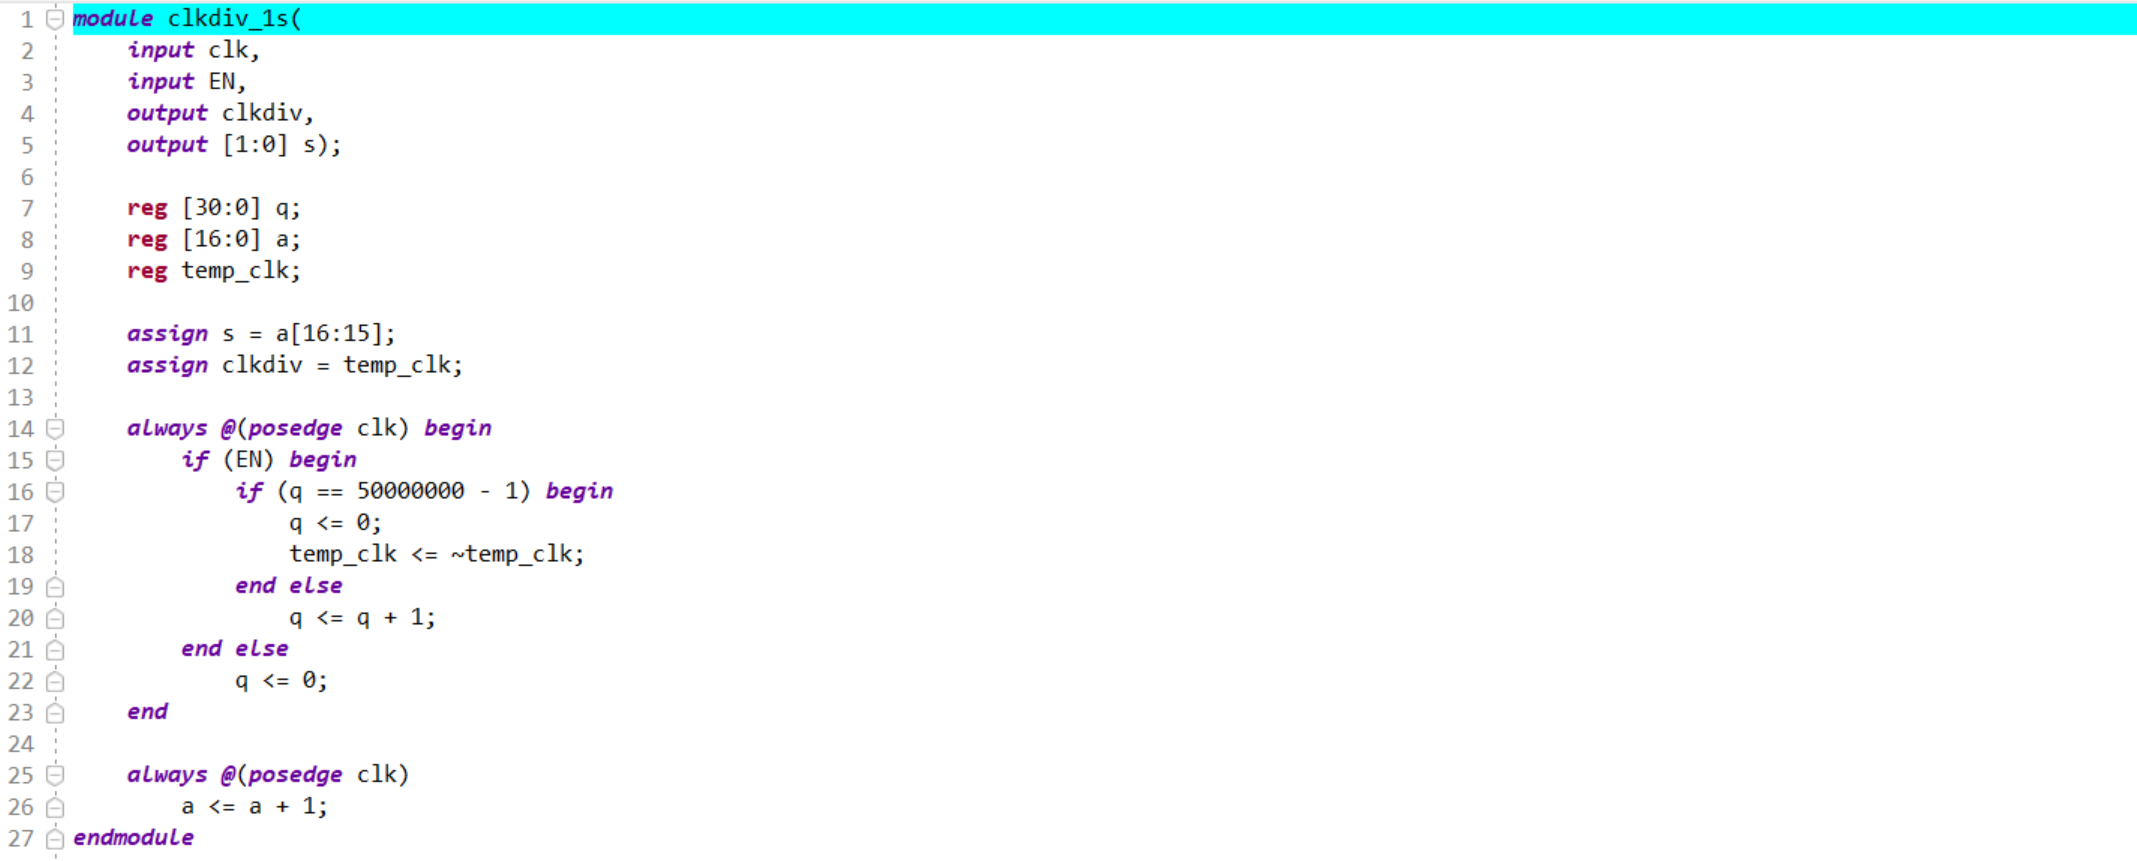
\includegraphics[width=1\textwidth]{clkdiv_1s_code.png}



\subsubsection{数码管显示模块 (traffic\_display)}
traffic\_display 模块的主要作用是根据状态信号 s 选择要显示的倒计时数值,并将其转换为7段数码管的显示格式,驱动数码管显示当前的倒计时。通过不断轮询显示主路和支路的高位和低位数值,实现倒计时的实时显示。

\vspace{1em}
\noindent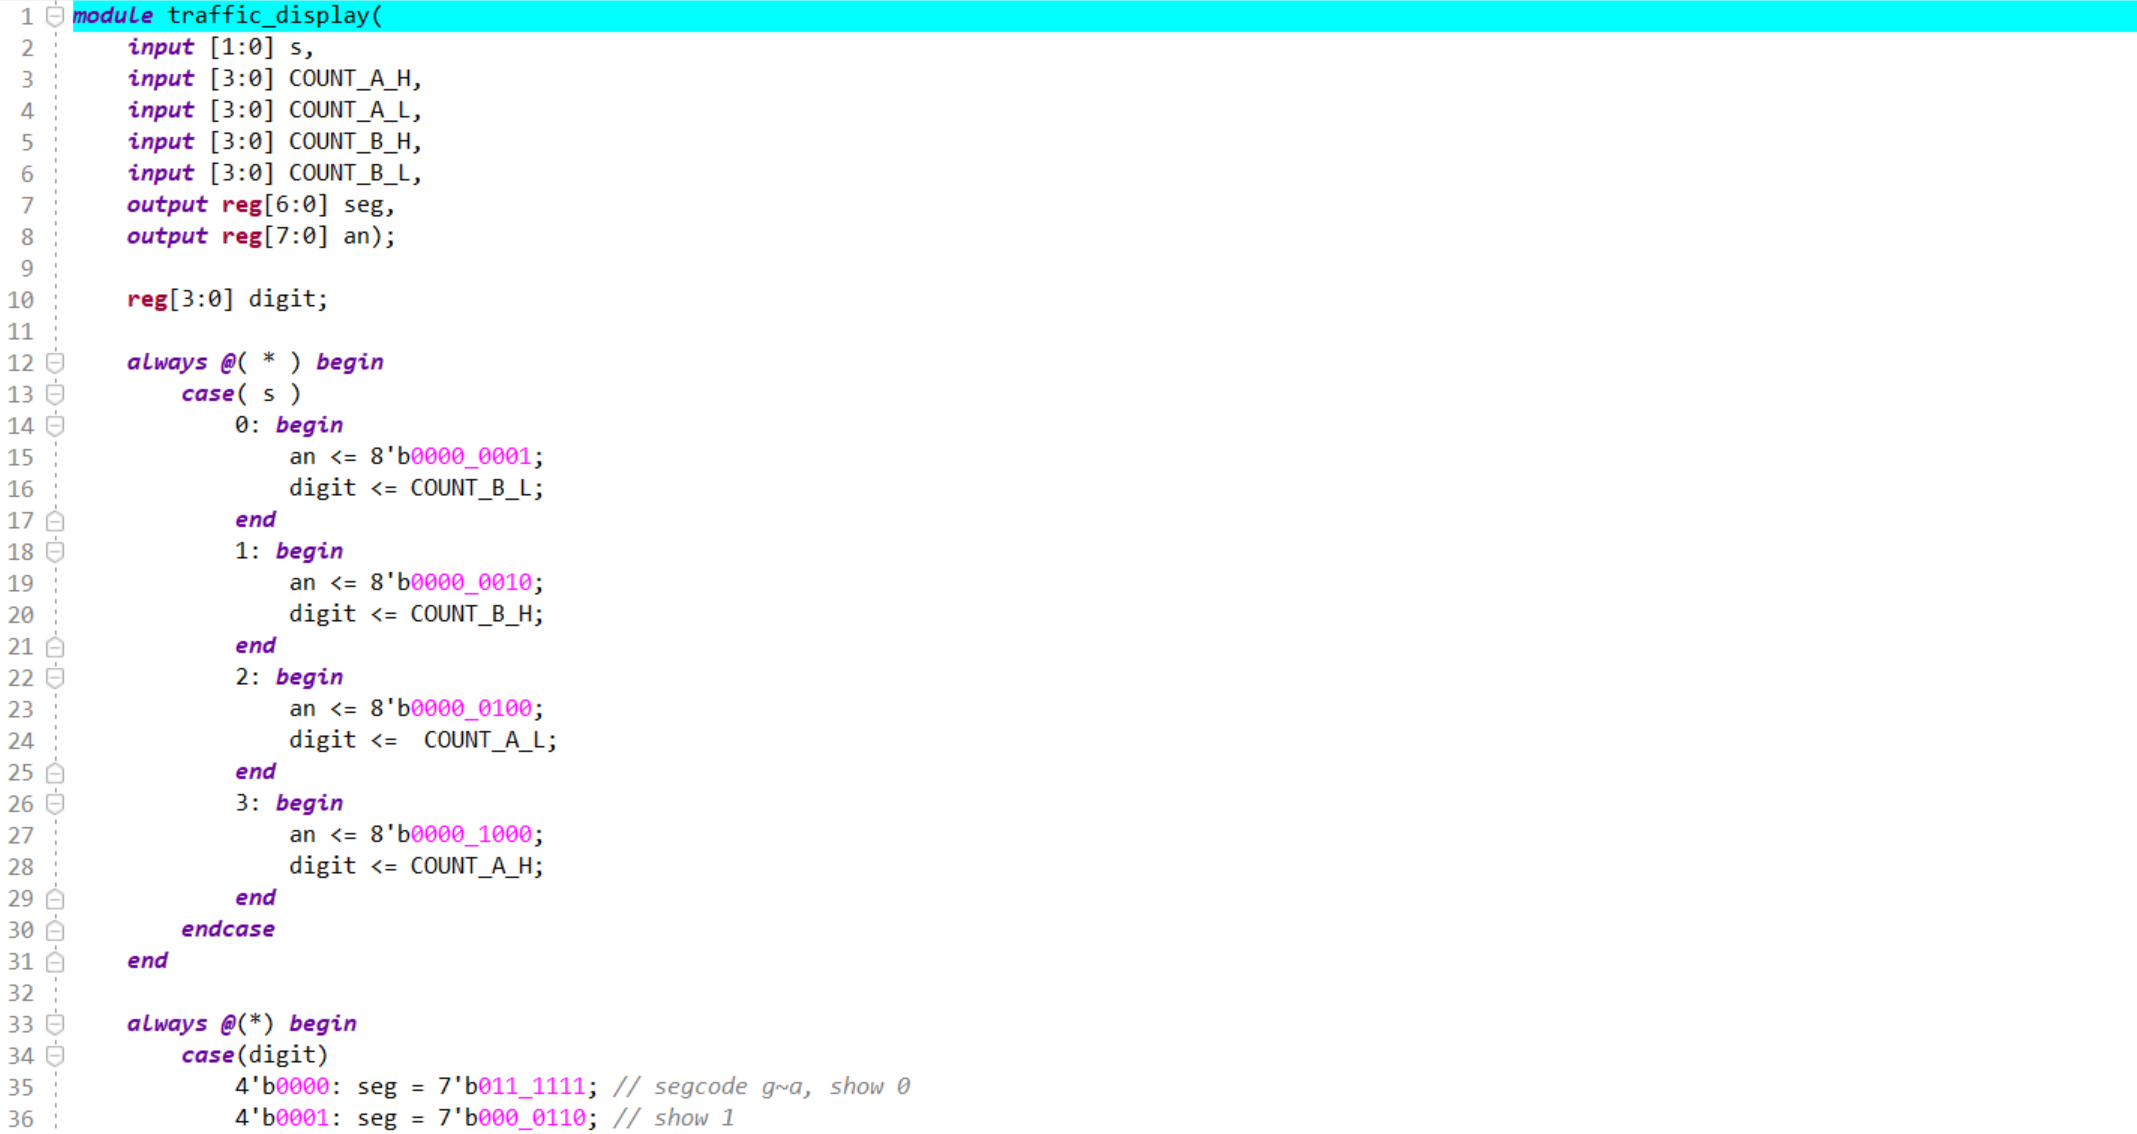
\includegraphics[width=1\textwidth]{traffic_display_1_code.png}
\noindent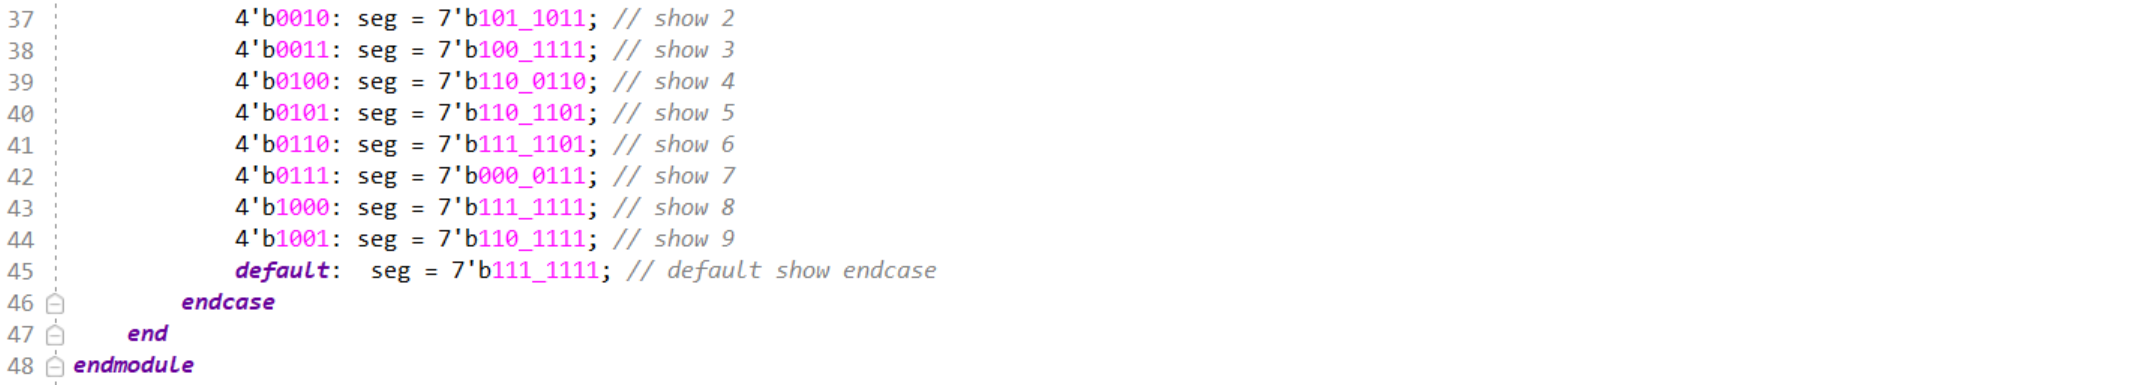
\includegraphics[width=1\textwidth]{traffic_display_2_code.png}

\subsection{配置文件编写}
\begin{enumerate}
    \item clk: 时钟输入信号,连接到 P17 引脚。
    \item EN: 使能信号,连接到 P5 引脚。
    \item LED\_main[0], LED\_main[1], LED\_main[2]: 主路的红、黄、绿灯,分别连接到 F6, G4 和 G3 引脚。
    \item LED\_secondary[0], LED\_secondary[1], LED\_secondary[2]: 支路的红、黄、绿灯,分别连接到 J4, H4 和 H3 引脚。
    \item an[0] 到 an[7]: 数码管位选信号,分别连接到 H1, C1, C2, G2, G6, E1, F1 和 G1 引脚。
    \item seg[0] 到 seg[6]: 数码管段选信号,分别连接到 B4, A4, A3, B1, B2, B3 和 C3 引脚。
\end{enumerate}

\vspace{1em}
\noindent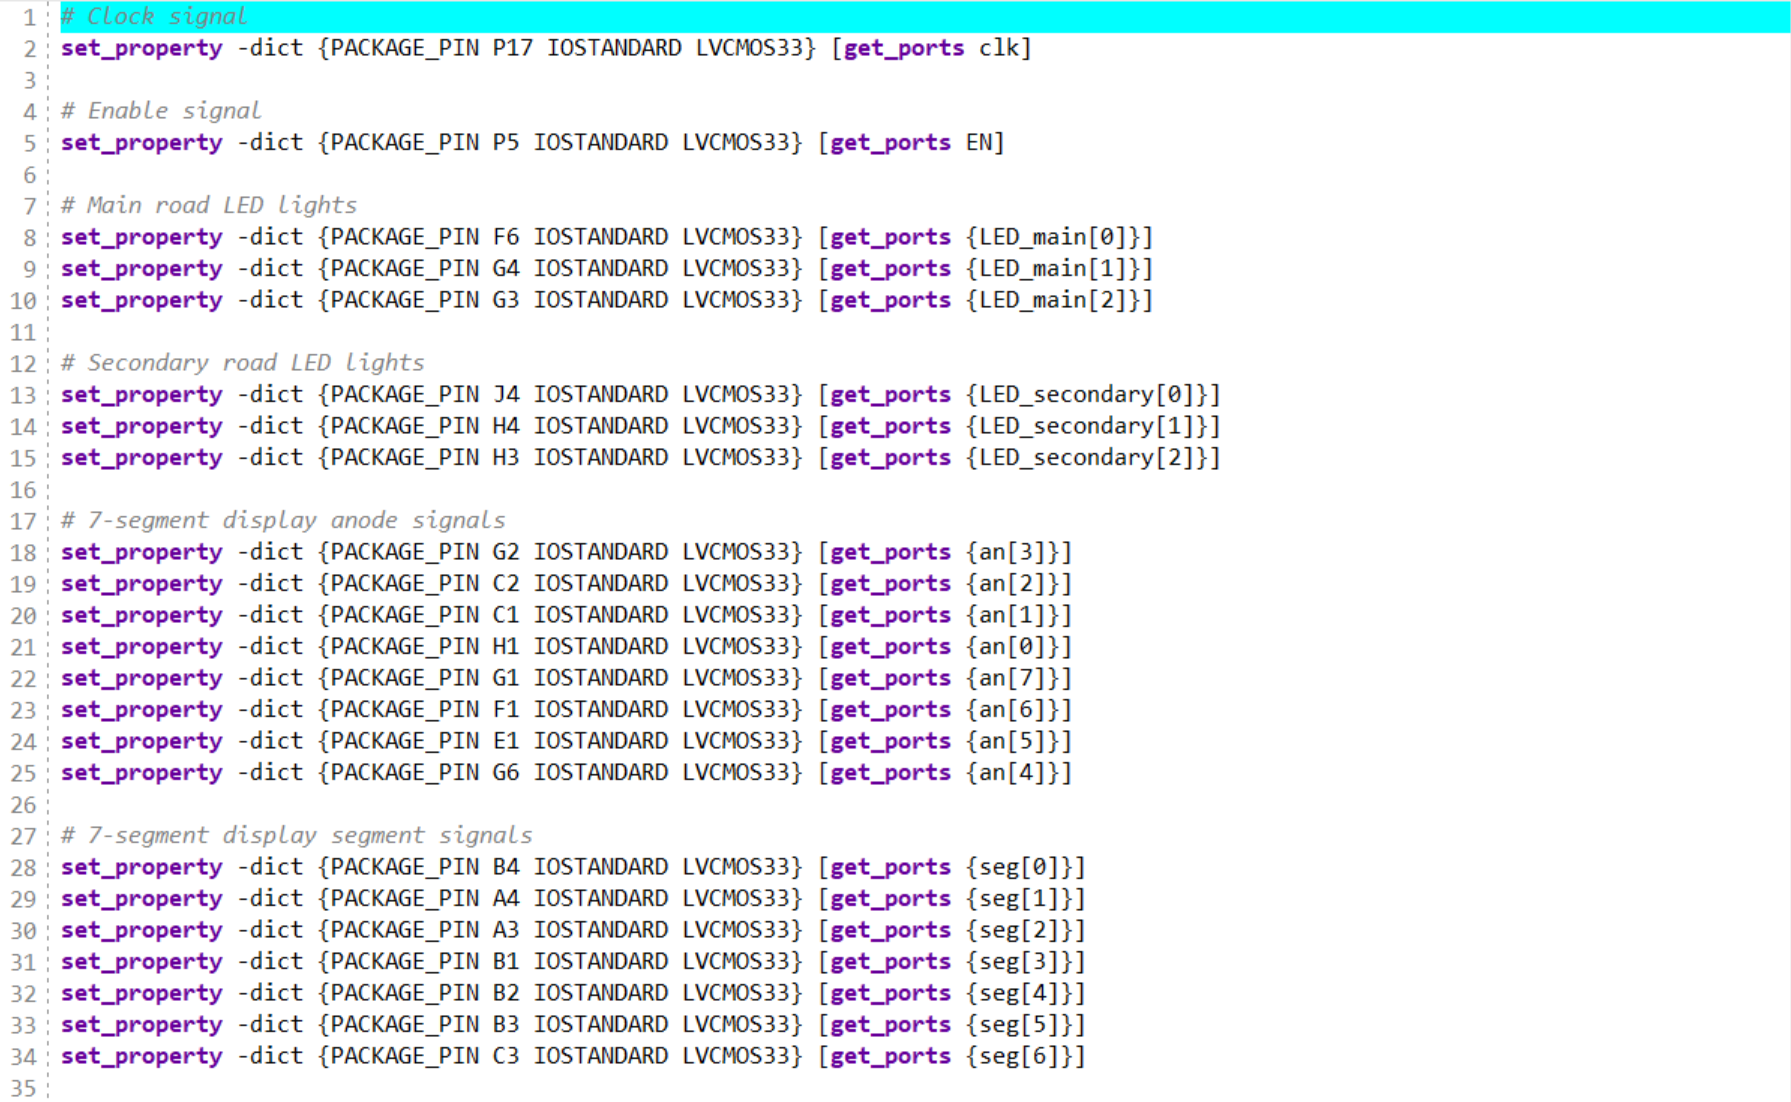
\includegraphics[width=1\textwidth]{constraint_code.png}


\newpage


\subsection{RTL分析与Program Device}

\paragraph{1.} RTL分析

\vspace{1em}

\noindent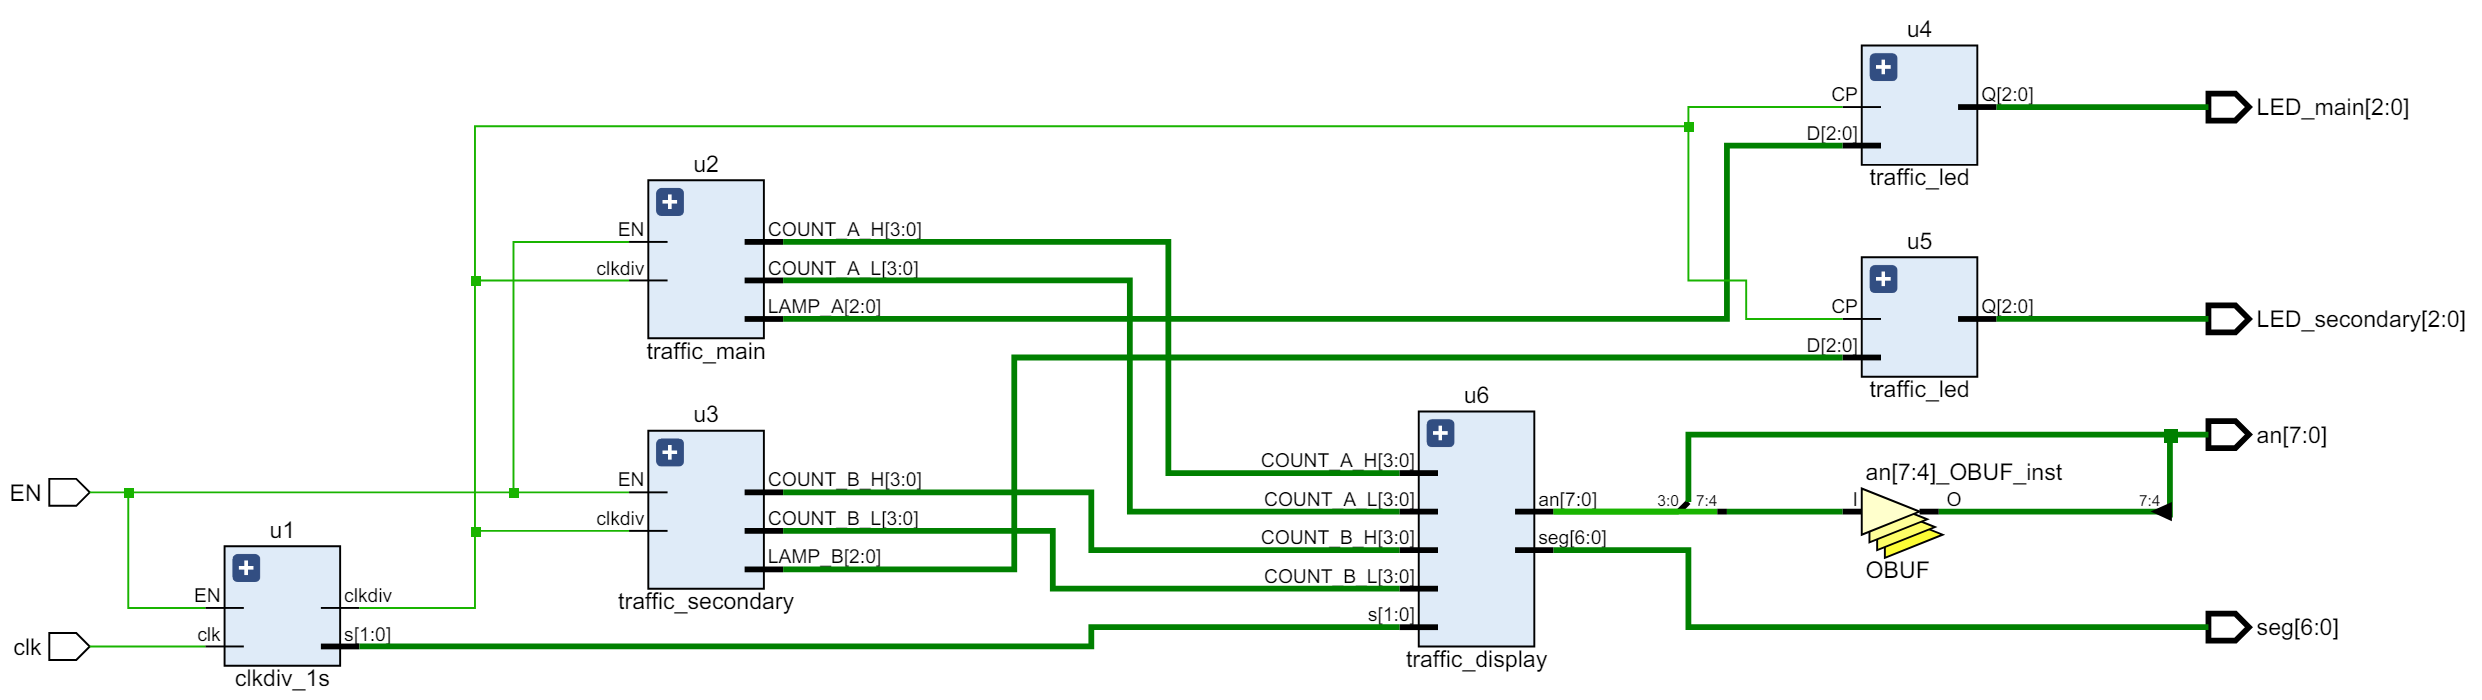
\includegraphics[width=1\textwidth]{schematic.png}


\paragraph{2.} Program Device

RTL分析、SIMULATION仿真分析验证功能实现无误后,通过SYNTHESIS、IMPLEMENTATION、Generate Bitstream以及Program Device步骤,成功在EGo1开发板上实现交通灯的功能。

\vspace{1em}

\begin{figure}[!h]
	\centering
	\begin{minipage}{0.49\linewidth}
		\centering
		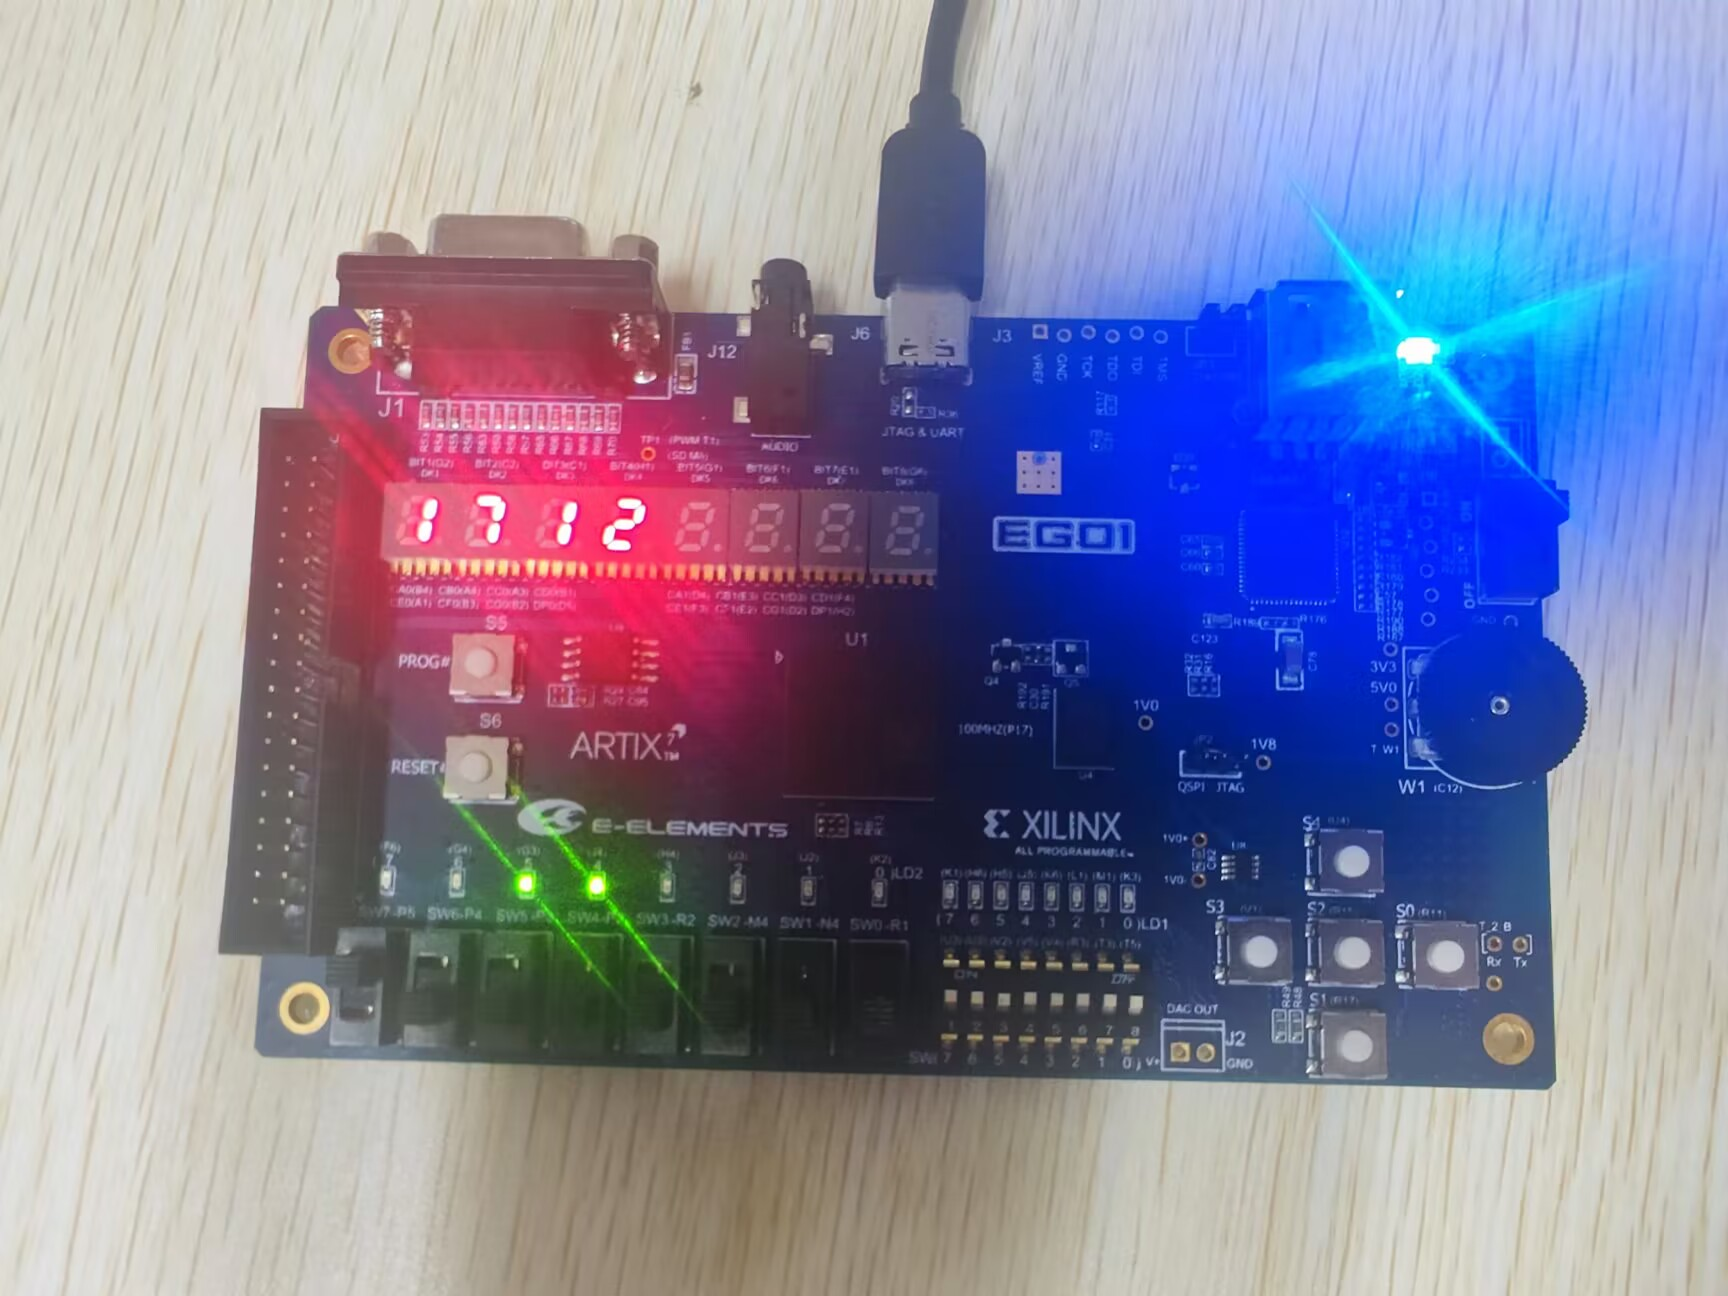
\includegraphics[width=0.8\textwidth]{program_device_pic_2.jpg}
	\end{minipage}
	\begin{minipage}{0.49\linewidth}
		\centering
		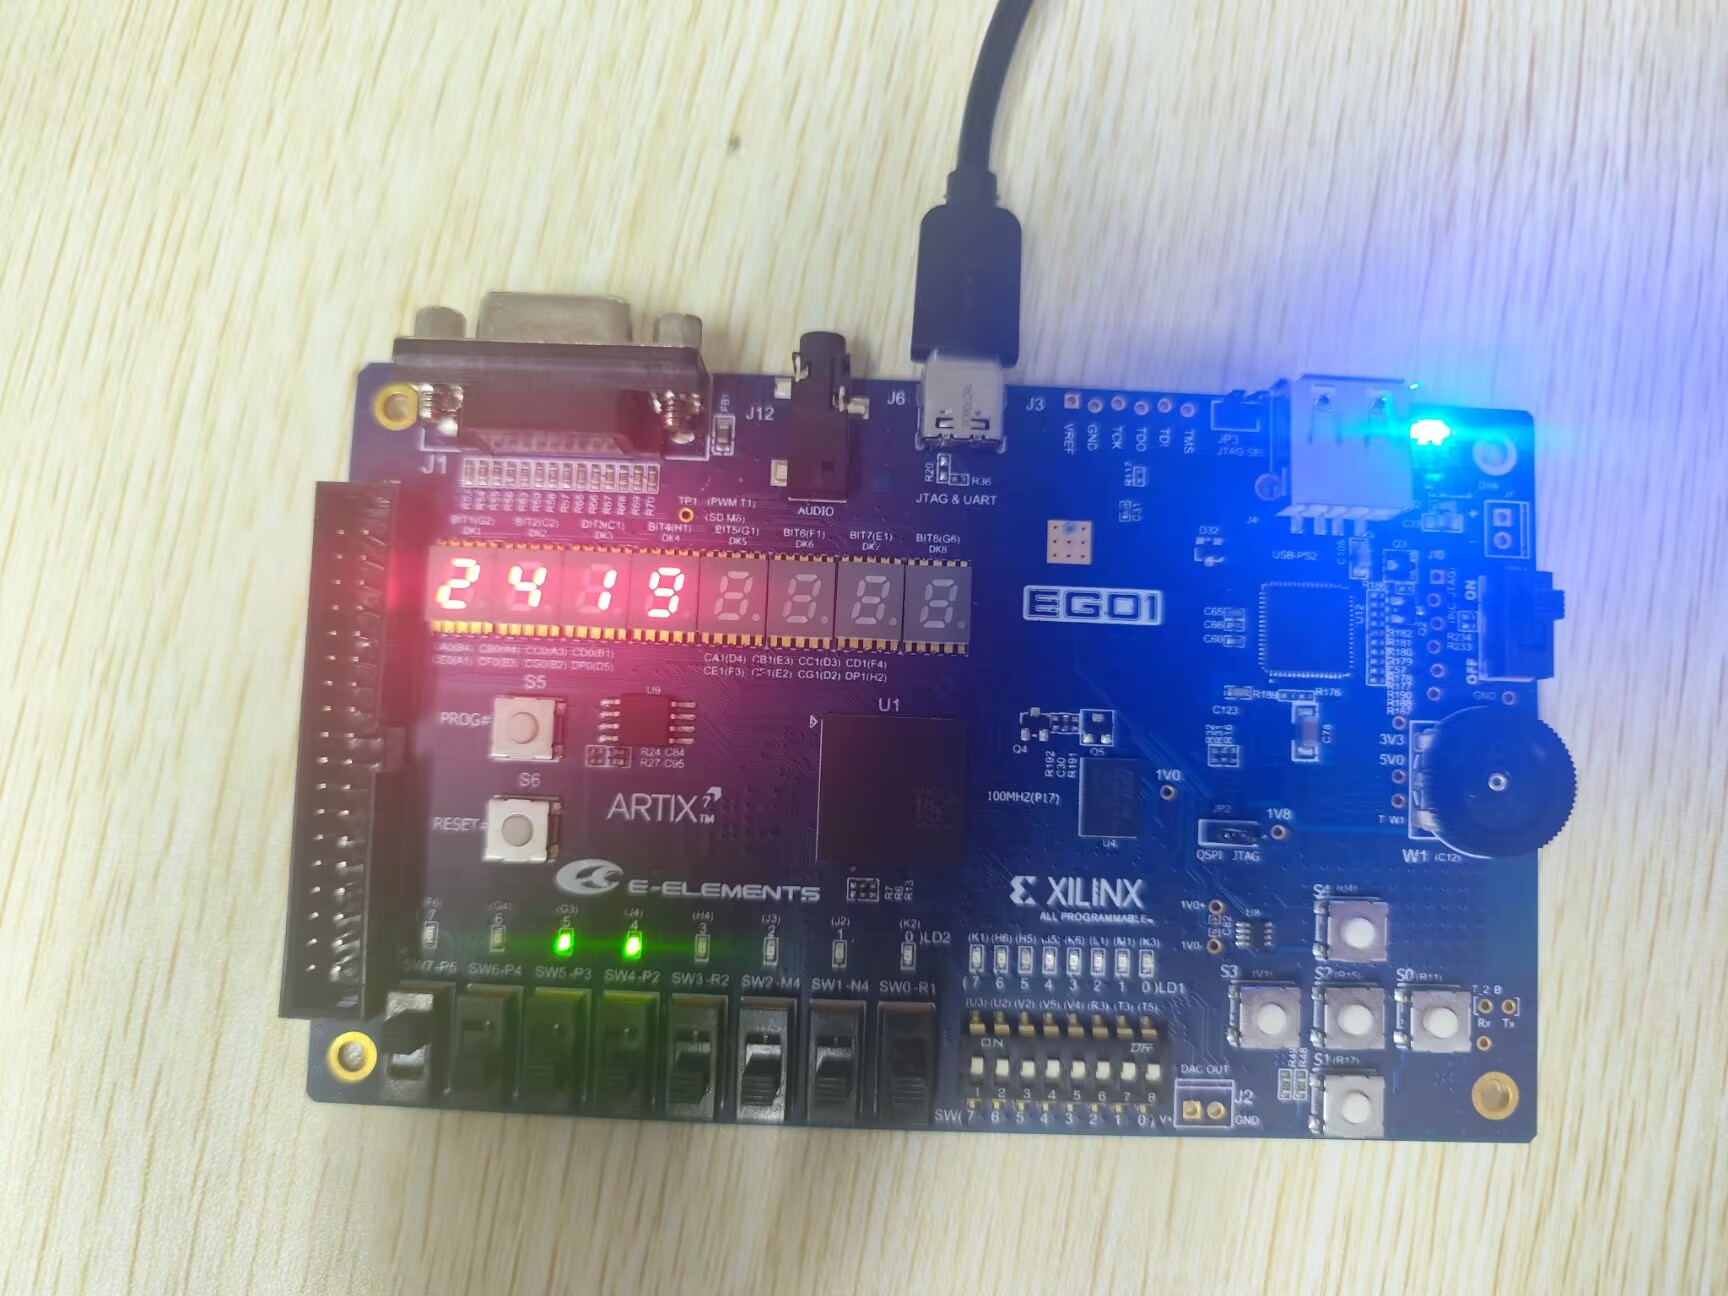
\includegraphics[width=0.8\textwidth]{program_device_pic_1.jpg}
	\end{minipage}
\end{figure}

\subsection{高级功能实现}
高级功能有两部分,一个是通过开关控制黄灯的闪烁,另一个是手动调整信号灯的时长。\textbf{这里我选择实现第二个功能}。第二个功能通过SET端控制。其中SET的配置文件这里不再赘述。同时,在traffic\_top模块中,调用重写后的traffic\_secondary\_set模块时添加了一个SET信号的映射。并且为traffic\_top添加输入端口和SET信号。


\subsubsection{手动调整信号灯时长}

为了实现能够手动调整信号灯的时长,这里仅实现对支路的信号灯进行调整。因此重写了traffic\_secondary模块,主要作用是实现支路交通灯的控制,并在需要时调整绿灯的时长。通过设置信号 SET 可以灵活调整绿灯的时长,以适应不同的交通情况。也就是说通过 SET 信号调整绿灯时长。使得支路的信号灯能够根据当前SET信号的状态设置倒计时,绿灯、黄灯和红灯的倒计时时长分别为 20/30 秒、5 秒和 35 秒。

模块中添加了一个内部变量green\_time和一个对SET信号敏感的部分,它会根据当前SET的状态为内部变量green\_time赋不同值,而内部变量green\_time会在切换到绿灯时赋值给绿灯的计时变量。

\vspace{1em}

\noindent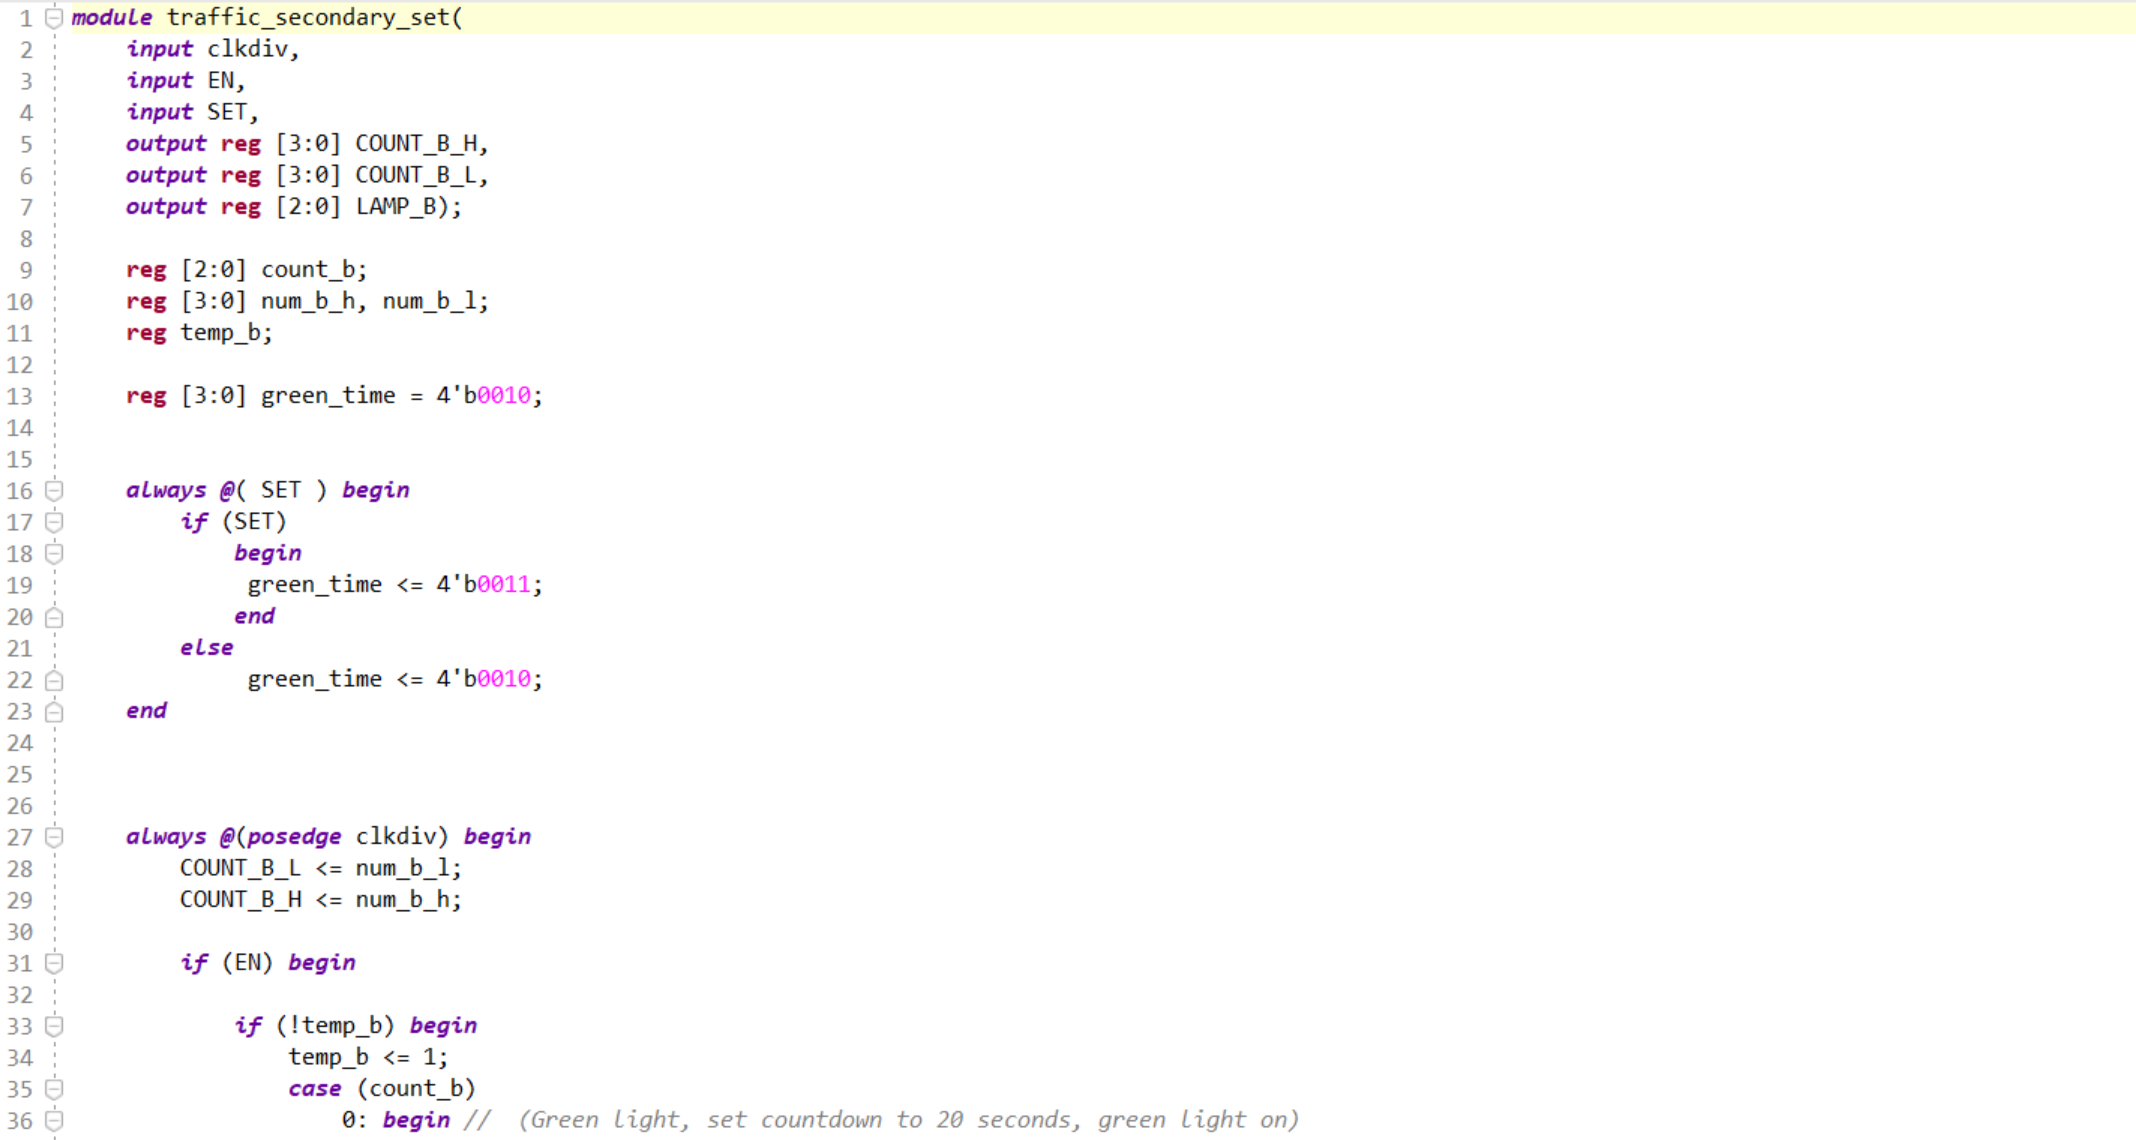
\includegraphics[width=1\textwidth]{traffic_secondary_set_1_code.png}
\noindent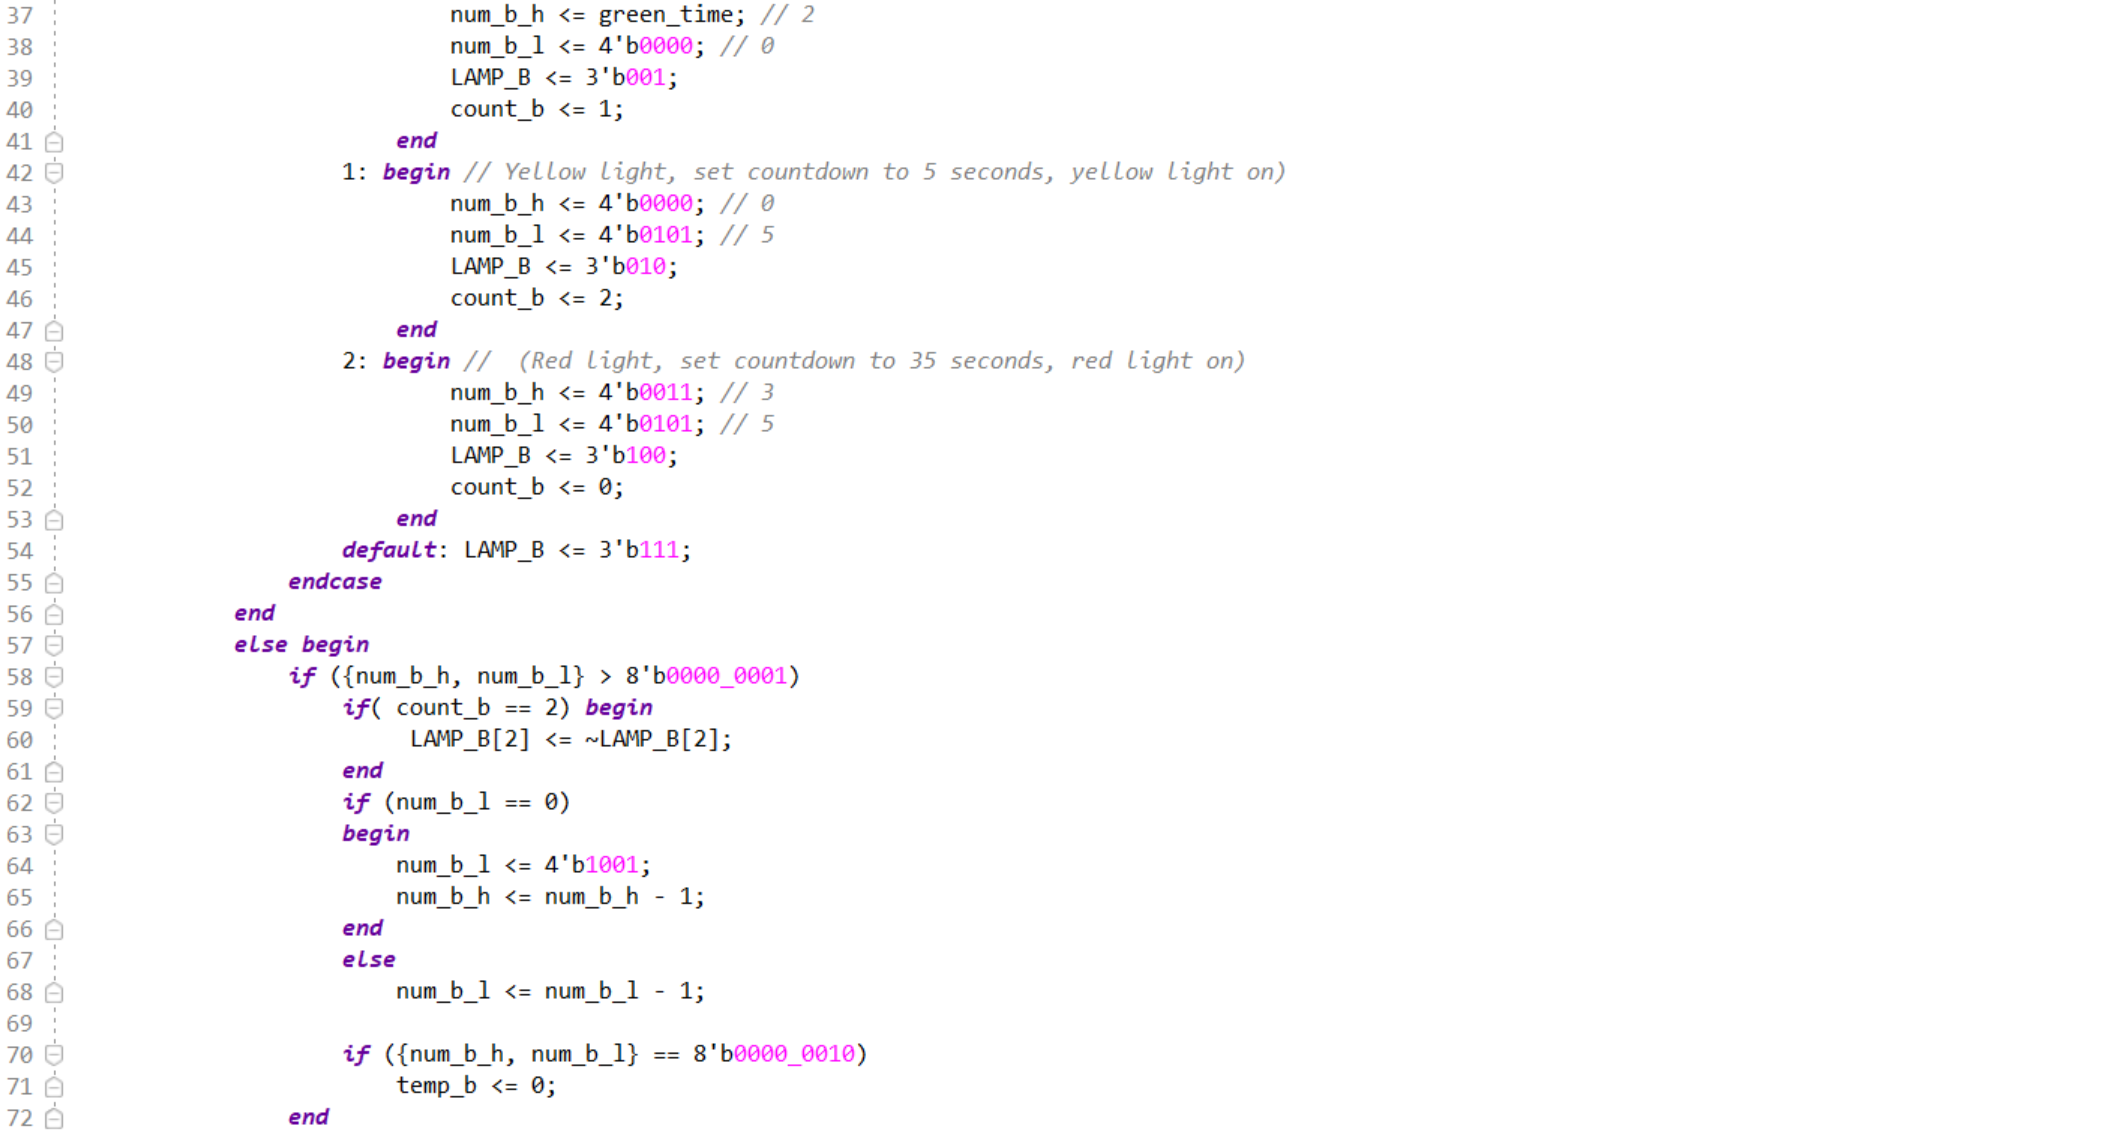
\includegraphics[width=1\textwidth]{traffic_secondary_set_2_code.png}
\noindent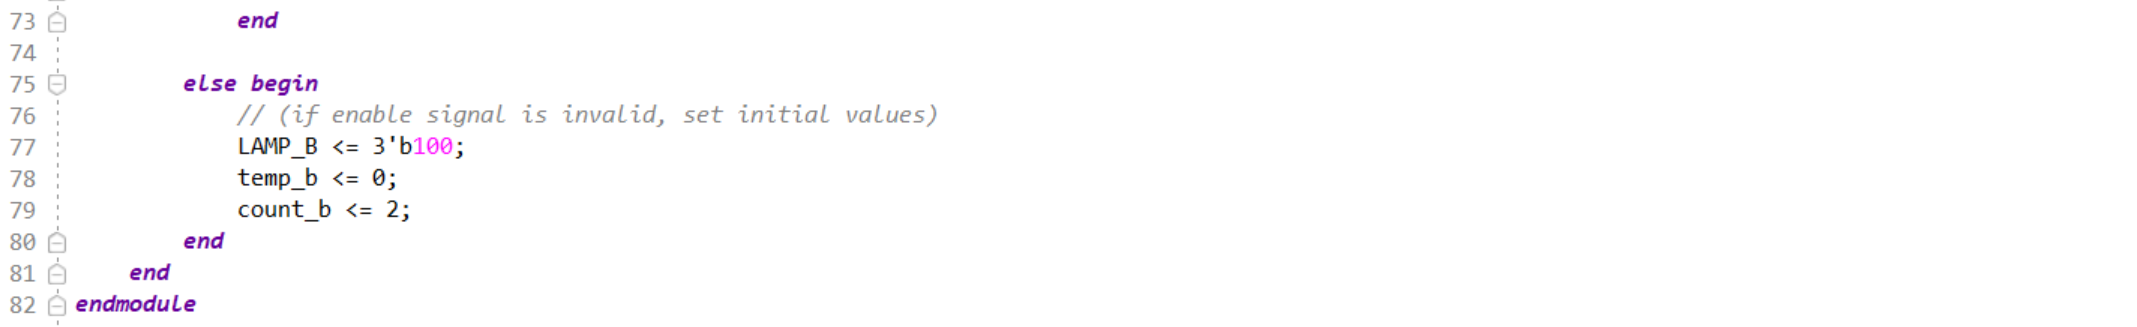
\includegraphics[width=1\textwidth]{traffic_secondary_set_3_code.png}






\section{调试和心得体会}

\subsection{调试过程}
在调试交通灯控制器时,我主要遵循以下几个步骤。首先确保所有代码模块在功能上都是独立的,并且通过仿真验证其正确性。我使用了Vivado工具进行RTL级别的分析和仿真测试,以确认代码逻辑的正确性。但是由于疏忽并没有注意时间复制的问题,导致直到硬件测试时,才发现代码逻辑上的错误,计时器在状态切换时没有正确重置,这导致了实际的倒计时与预期不符。针对这些问题,我对计时逻辑进行了修正,并在仿真中反复测试,确保计时器在每个状态切换时都能正确工作。

为了实现高级功能,我分别设计了对应的模块,并通过仿真和硬件测试进行验证。在夜间模式下,黄灯能够按预期闪烁;在手动调整信号灯时长时,能够通过开关信号灵活控制绿灯的时长。


\subsection{心得体会}
通过本次实验,我深刻体会到Verilog编程和FPGA开发的复杂与挑战。首先Verilog语言的硬件描述特性要求我们在设计时必须考虑硬件实现的具体逻辑,而不仅仅是软件编程的思维。这种思维方式的转变,使我在编写代码时更加注重时序逻辑和信号的传递,确保每个模块的功能都能在实际硬件中正确实现。

调试过程中遇到的各种问题,让我更加明白硬件设计中细节的重要性。每一个小的错误,都可能在硬件实现中被放大,影响整体系统的稳定性。因此,在设计和调试过程中,必须要细致入微,逐步验证每一个功能模块,确保其独立正确性,然后再进行整体集成测试。

在硬件测试阶段,通过实际操作FPGA开发板,进一步加深了我对数字电路和硬件实现的理解。与软件仿真不同,硬件测试能够暴露更多实际运行中的问题,这些都是在仿真中无法完全体现的。通过硬件测试,我学会了如何识别和解决这些实际问题,提升了我在硬件开发中的实践能力。

通过实现高级功能,让我更好地掌握了Verilog编程技巧,提高了我在系统设计中的创新能力。这些功能的实现,进一步增强了系统的实用性和灵活性,也让我在实验中获得了极大的成就感。这次实验不仅让我掌握了交通灯控制器的设计与实现方法,也让我在实际操作和调试中积累了丰富的经验。这些宝贵的经验和技能,将对我今后的学习和工作产生深远的影响。

\end{document}
